\tikzstyle{node}=[rectangle,draw=blue!50,fill=blue!20,thick,text width=1.5cm,text centered,font=\footnotesize]
\tikzstyle{smallnode}=[rectangle,draw=blue!50,fill=blue!20,thick,text width=1cm,text centered,font=\footnotesize]
\tikzstyle{pre}=[<-,shorten <=-3pt,>=stealth,thick]
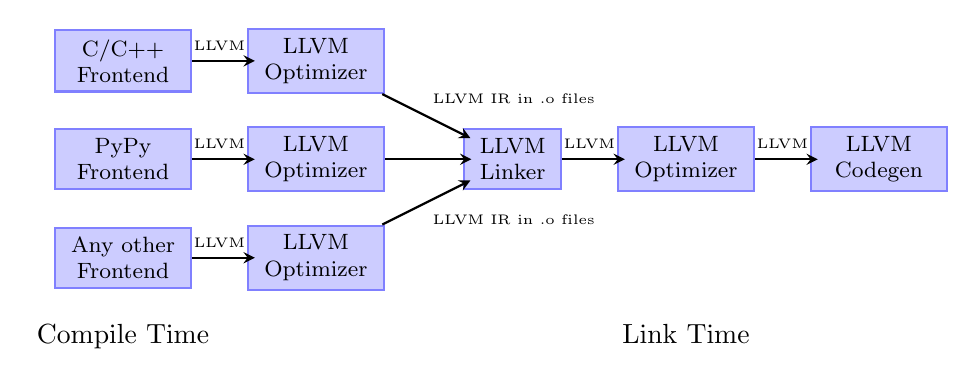
\begin{tikzpicture}
        \node[node] (cfe)                                       {C/C++ Frontend};
        \node[node] (pyfe)  [below of=cfe,   node distance=1.25cm] {PyPy Frontend};
        \node[node] (anyfe) [below of=pyfe,  node distance=1.25cm] {Any other Frontend};

        \node[node] (opt1)  [right of=cfe,   node distance=2.45cm] {LLVM Optimizer}
         edge[pre] node[auto,swap] {\tiny{LLVM}} (cfe);
        \node[node] (opt2)  [right of=pyfe,  node distance=2.45cm] {LLVM Optimizer}
         edge[pre] node[auto,swap] {\tiny{LLVM}} (pyfe);
        \node[node] (opt3)  [right of=anyfe, node distance=2.45cm] {LLVM Optimizer}
         edge[pre] node[auto,swap] {\tiny{LLVM}} (anyfe);

        \node (compiletime) [below of=anyfe, node distance=1cm]    {Compile Time};
         
        \node[smallnode] (llvmlinker) [right of=opt2, node distance=2.5cm] {LLVM Linker}
         edge[pre] node[auto,swap] {\tiny{LLVM IR in .o files}} (opt1)
         edge[pre]                                              (opt2)
         edge[pre] node[auto]      {\tiny{LLVM IR in .o files}} (opt3);

        \node[node] (llvmopt)      [right of=llvmlinker, node distance=2.2cm] {LLVM Optimizer}
         edge[pre] node[auto,swap] {\tiny{LLVM}} (llvmlinker);
        \node[node] (llvmcodegen)  [right of=llvmopt,    node distance=2.45cm] {LLVM Codegen}
         edge[pre] node[auto,swap] {\tiny{LLVM}} (llvmopt);

        \node[anchor=base] (linktime) at(llvmopt.base |- compiletime.base)     {Link Time};
     \end{tikzpicture}